\documentclass{report}
\usepackage{cite}
\usepackage{titlesec}
\usepackage{amsmath}
\usepackage[english]{babel}
\usepackage{caption}
\usepackage{multirow}
\usepackage{tikz}
\usepackage{amsmath}
\usepackage{amssymb}
\usetikzlibrary{calc}
\usetikzlibrary{arrows}
\usepackage{pgfplots}
\captionsetup[figure]{font=small}	
\captionsetup[table]{font=footnotesize}
\newcommand{\R}{\mathbb{R}}
\usepackage{float}
\tolerance=1
\emergencystretch=\maxdimen
\hyphenpenalty=10000
\hbadness=10000
\usepackage{array}
\usepackage{textgreek}
\usepackage{graphicx}
\graphicspath{ {./images/} }

\begin{document}


\begin{titlepage}
\begin{center}
\vspace*{0.8cm}
\begin{figure}[H]
\centering

\includegraphics[width=0.4\textwidth]{logo_uni}
\end{figure}
\LARGE{\textsc{University of Padua}}\\
\vspace*{0.1cm}
\Large{\textsc{Department of Information Engineering}}\\
\vspace*{1.0cm}
\Large{\textsc{Information Security Report}}\\
\vspace*{0.1cm}
\Large{\textsc{Laboratory Session 2}}\\
\vspace*{0.8cm}
\huge{\textbf{Implementation of random binning encoding and secrecy rate
evaluation}}\\
\vspace*{1cm}
\end{center}
\large{\textit{Author:}}
\hfill
\large{\textit{Teacher:}} \\
\large{ZANON \textsc{ALBERTO}}
\hfill
\large{Nicola \textsc{Laurenti}}\\
\large{MICHELON \textsc{LUCA}}\\
\large{SCREMIN\textsc{ NICOLA}}\\
\large{NIKHIL \textsc{KARAKUCHI CHIDANANDA }}\\
\large{PORRO \textsc{THOMAS}}\\

\vspace*{0cm}
\begin{center}
\large{29 November 2020}\\
\end{center}
\end{titlepage}
\pagebreak


\setcounter{page}{1}
\pagenumbering{arabic}
\chapter*{Solution}
\par Our solution to laboratory 2 is entirely implemented using Python. Specifically, we made use of the {\tt NumPy} library to easily manipulate vectors and quickly compute operations between them. The solution is composed of 8 Python source files: {\tt main.py} contains all the function for tasks, {\tt task1.py} contains functions necessary to carry out the implement the wiretap channel, so that it accepts an
input  and produces the corresponding pair of outputs (y; z), {\tt task2.py} contains random encoder function to implement the random binning encoder, so that it accepts an input and produces the corresponding output, {\tt task3.py} contain random decoder function to implement the legitimate decoder, so that it accepts an input and produces the corresponding output,  {\tt task4.py} contains the functions implement the encoder + eavesdropper channel, {\tt task5.py}  contains function to implement the wiretap BSC, {\tt task6.py} contains functions for repeat the simulations in Tasks 3-4 with the wiretap BSC, evaluate the resulting reliability in terms of Bob's error rate on the secret message chain P, evaluate the resulting the secrecy in terms of leaked information to Eve on the secret message I and compute an upper bound to the mechanism security in terms of distinguishability from the ideal
counterpart and {\tt utils.py} contains function to convert the string to array and the array to string. 
 \section*{Task 1}
\par We implemented the uniform error channel using the function {\tt legittimate\_channel(x)} the legitimate channel introduces at most 1 binary error per word,
 Legitimate a random integer for choosing which is the error and XOR with the the input and {BitArray(bin=errors[index]).uint} transforms binary string to integer. and {\tt eve\_channel(x)} for the eavesdropper channel introduces at most 3 binary error per word, and the {\tt main()} function contains the variables  x = "01001000"
  y = []
  z = []
  contyz = 0
  conty = 0
  contz = 0
  n = 25000 after that we call the function  {\tt legittimate\_channel(x)} and adds new word to a list y.append(word\_y) and Same for Eve by  calling {\tt eve\_channel(x)} after the all list is appended we Verify the conditional independence and uniformity and print the output and plot the graphic for Legitimate channel and plot the graphic for Eavesdropper channel. \hfill \break \linebreak  Verify the conditional independence and uniformity of our outputs, P(y,z|x) = P(y|x)*P(z|x), in our experiment we used y = 64 and z = 4 (chosen randomly). We obtained following results:  \hfill \break
    \linebreak
  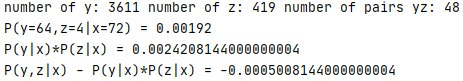
\includegraphics[width=13cm,height=2cm]{output1}
  \linebreak And we iterated our algorithm 25 000 times and we get this output.\hfill \break
   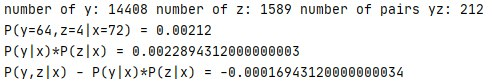
\includegraphics[width=13cm,height=2cm]{output2} \hfill \break
  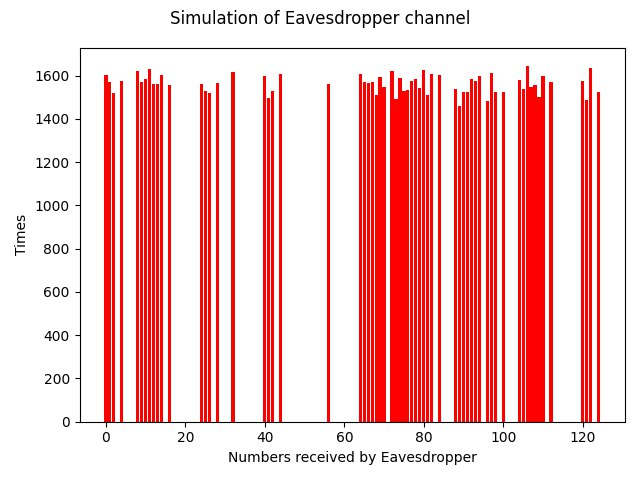
\includegraphics[width=10cm,height=7cm]{1} \linebreak
 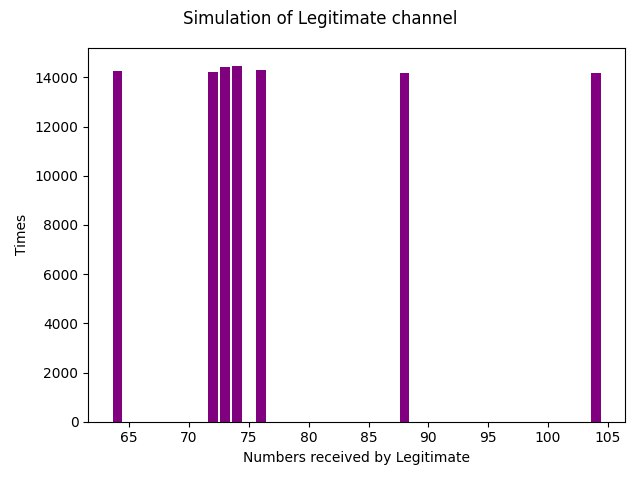
\includegraphics[width=10cm,height=7cm]{2}
  \section*{Task 2}
  In task 2 we are using the random lib for Generate pseudo-random numbers and BitArray lib for efficient arrays of booleans for better implementation, we defined X array variable for storing the codewords, and {\tt rand\_encoder(d)} function for Implement the random binning encoder, first we checks which codeword starts with the prefix and gets it and Calculates the complement of the binary given as input and the codeword x is chosen randomly and uniformly within the bin associated to the message u, to optimise the code we could compute the complement if, and only if, the rand == 1, in this i preferred to show the two choices and how the randomness choice it.
\section*{Task 3}
In task we are using the {\tt Numpy} and {\tt BitArray} for array operations {\textit G}  is a 4 linear independent codewords (as columns)
first 4 rows form the identity matrix 4x4 and {\textit H} is the parity check matrix built starting from G last 3 rows of G + Identity 3x3 {\textit coset\_leader} look-up table for choosing the coset leader of the syndrome computed in a paper using H and all of possible choices of 3 bits [x x x], {\textit inputs} is all of possible inputs, and {\tt rand\_decoder(y\_string)} is function for implement the legitimate decoder, so that it accepts an
input and produces the corresponding output.
\section*{Task 4}
Here in task 4 the tasks are divided into two parts first part we are using 8X128 matrix to collect the statistics of PDM , pz|u after that we are running simulations by sending the message through the eavesdropper branch of the channel and thereby collecting the distribution  pz|u, then we will plot the result with the Number as x and Probability as y axis using z\_pmds[i], Here the message(u) is not taken randomly so we are estimating the distribution pz|u. \hfill \break \linebreak
 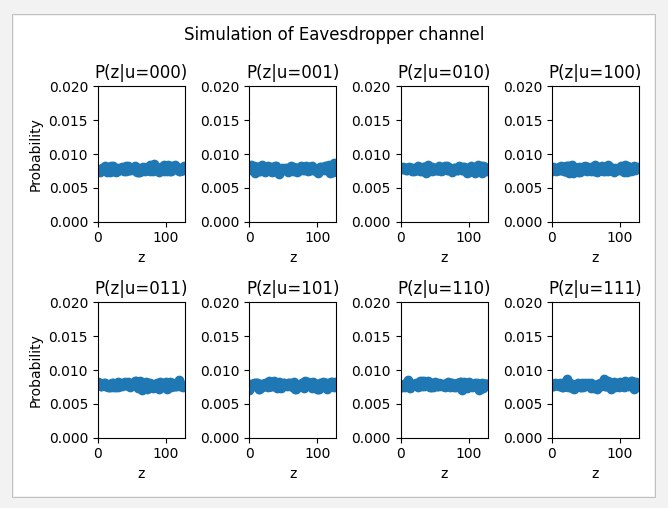
\includegraphics[width=10cm,height=7cm]{4}  \hfill \break \linebreak
In the second part ,we are running some simulations  by taking a random message and observe the  z received by the eavesdropper. Here both u and z are random variables.Then we collect the distribution pu|z .After that we compute the marginal distribution, entropies and the mutual information and we use the help function to compute the following rand\_encoder(), eve\_channel().

\section*{Considerations and remarks}
1) How many secret message bits per channel use ("transmitted word") have you obtained with your
scheme?
How many secret bits per binary digit ("transmitted bit")?  \hfill \break \linebreak
Because the legitimate channel introduce at most 1 error and we can always detect it and find the correct input. the eve channel can generate at most 3 errors, he wont understand which bit was ‘flipped’. \hfill \break  \linebreak
2) Is it possible to obtain 4 secret bits per channel use?
If so, how should you change your encoder/decoder? If not, why? \hfill \break \linebreak
No, we cannot have more secrets bits than we have sent as input \hfill \break \linebreak
3) Is it possible to obtain 2 secret bits per channel use?
If so, how should you change your encoder\/decoder? If not, why?  \hfill \break \linebreak
Yes because at most we have 3 secure bits (upper-bound), maybe having a deterministic encoder\/decoder? (don't know)\hfill \break \linebreak
4)One could consider evaluating the secrecy of this mechanism by cascading the eavesdropper channel
with a decoder and measuring the resulting error rates. What do you expect Eve's error would be?
Why resort to (more complicated) evaluating the mutual information? \hfill \break \linebreak
Since Eve cannot know which bits are flipped, we suppose that Eve has to choose randomly among all possibility (1\//2\^3). So the error is 1-1\//2\^3
\section*{Task 5}
In task 5 we are using NumPy, bitstring, utils for string to array and array to string, math, matplotlib for plot and statistics libraries for better implementation and we import the task2 and task3 to connected in between the random binning encoder developed in Task 2, and the decoder
developed in Task 3, for test with task 2/3 encoder decoder we defined deltas as np.arange(0, 1.1, 0.1), epsilon  as 0.1, wrong\_eves to store number of wrong codewords decoded by eve in percentage, wrong\_bobs to store number of wrong codewords decoded by bob in percentage, codeword\_error\_eve for \% of wrong bits in the codeword received by eve after we compute the channel capacity then we defined     multi\_error\_codeword\_count to count how many pairs of codewords (x, y)have more than 1 bit different, error\_bob\_count for wrong codewords decoded by bob and this is not the same as multi\_error\_codeword\_count, because the complementary (+- 1 bit) of the codewords are decoded correctly, error\_eve\_count for wrong codewords decoded by eve and codeword\_error\_eve\_cycle to count how many flipped bits are in the codeword received by eve at each cycle after that repeat multiple times for better estimates then compare decode with input.\hfill \break \linebreak

Task 5 is a binary symmetric channel that flips bits in bob and eve channels with probability epsilon and delta. The bits to flip are chosen uniformly in the input with a simple random generation of 0 and 1, where 1 means that a flip will occur in that position. This mask is applied with a XOR.
The channel is tested first with a long string of bits and the number of flipped bits equals in percentage the values provided for epsilon and delta.
Then the full range of inputs for the encoder and decoder of task 2 and 3 is tested multiple times and the results are averaged for better accuracy.
The results show that with sufficiently high values of epsilon bob's decoder can fail as more than 1 bit is flipped and the Hamming code can, at most, correct one error. The message decoded by eve depends on the input codeword and delta.
The code logs both wrong decoded codewords and the number of flipped bits in the output channels, to provide an insight of the decoding mechanism that relies also on the complementary of the input codewords.
Two plots are provided at the end to show these results, by enabling the corresponding if statement.

\section*{Task 6}

Here in task 6 for Evaluate the system security over the wiretap BSC we use the values\_e variable for \textepsilon \space and values\_d for \textdelta \space then Repeating task 3 and computing reliability of Bob 


\end{document}

